\documentclass[tikz,border=5pt]{standalone}
\usepackage{pgfplots}
\usepgfplotslibrary{groupplots}
\pgfplotsset{compat=1.18}

\definecolor{corba}{HTML}{365FB3}
\definecolor{punt}{HTML}{B91C1C}
\definecolor{assimptota}{HTML}{6B7280}

\begin{document}
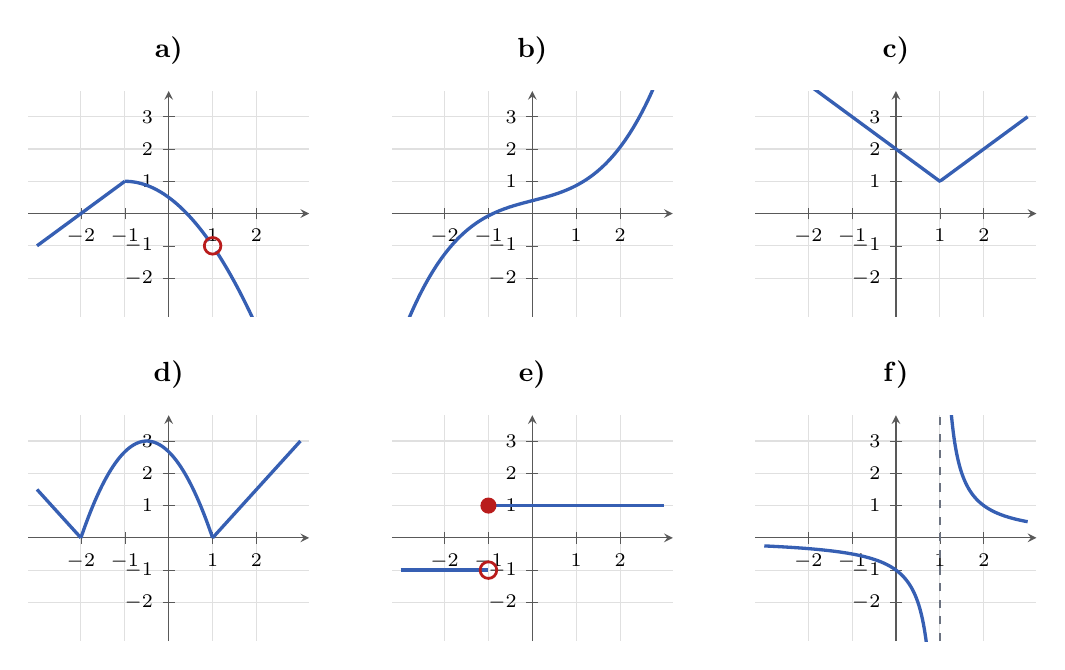
\begin{tikzpicture}
  \begin{groupplot}[
    group style={group size=3 by 2, horizontal sep=1.05cm, vertical sep=1.25cm},
    width=5.15cm,
    height=4.45cm,
    axis lines=middle,
    xmin=-3.2,
    xmax=3.2,
    ymin=-3.2,
    ymax=3.8,
    xtick={-2,-1,0,1,2},
    ytick={-2,-1,0,1,2,3},
    tick label style={font=\scriptsize},
    grid=major,
    grid style={black!12},
    axis line style={black!65},
    tick style={black!65},
    clip=true,
  ]
    % a) Punt angulós en x=-1 i forat en x=1.
    \nextgroupplot[title={\textbf{a)}}]
      \addplot[corba, very thick, domain=-3:-1, samples=80] {x+2};
      \addplot[corba, very thick, domain=-1:0.92, samples=80]
        {1-0.5*(x+1)^2};
      \addplot[corba, very thick, domain=1.08:2.55, samples=70]
        {1-0.5*(x+1)^2};
      \addplot[
        only marks,
        mark=o,
        mark size=3pt,
        mark options={draw=punt, fill=white, line width=1pt}
      ] coordinates {(1,-1)};

    % b) Funció polinòmica suau.
    \nextgroupplot[title={\textbf{b)}}]
      \addplot[corba, very thick, domain=-3:3, samples=150]
        {0.12*x^3+0.35*x+0.4};

    % c) Punt angulós desplaçat.
    \nextgroupplot[title={\textbf{c)}}]
      \addplot[corba, very thick, domain=-2.7:3, samples=140]
        {abs(x-1)+1};

    % d) Dos punts angulosos: el de l'esquerra és (-2,0).
    \nextgroupplot[title={\textbf{d)}}]
      \addplot[corba, very thick, domain=-3:-2, samples=60]
        {-1.5*(x+2)};
      \addplot[corba, very thick, domain=-2:1, samples=100]
        {-(4/3)*(x+2)*(x-1)};
      \addplot[corba, very thick, domain=1:3, samples=60]
        {1.5*(x-1)};

    % e) Discontinuïtat de salt en x=-1.
    \nextgroupplot[title={\textbf{e)}}]
      \addplot[corba, very thick, domain=-3:-1, samples=40] {-1};
      \addplot[corba, very thick, domain=-1:3, samples=40] {1};
      \addplot[
        only marks,
        mark=o,
        mark size=3pt,
        mark options={draw=punt, fill=white, line width=1pt}
      ] coordinates {(-1,-1)};
      \addplot[
        only marks,
        mark=*,
        mark size=2.7pt,
        mark options={draw=punt, fill=punt}
      ] coordinates {(-1,1)};

    % f) Funció racional amb asímptota vertical en x=1.
    \nextgroupplot[title={\textbf{f)}}]
      \addplot[assimptota, dashed, thick] coordinates {(1,-3.2) (1,3.8)};
      \addplot[corba, very thick, domain=-3:0.78, samples=150]
        {1/(x-1)};
      \addplot[corba, very thick, domain=1.22:3, samples=150]
        {1/(x-1)};
  \end{groupplot}
\end{tikzpicture}
\end{document}

